% Internal pre-results manuscript.  Empirical cells are intentionally blank.
\documentclass[sigconf,anonymous]{aamas}
\usepackage{amsmath}
\usepackage{booktabs}
\usepackage{array}
\usepackage{url}
% Copyright and conference block copied from the official AAMAS 2027 sample.
\makeatletter
\gdef\@copyrightpermission{
  \begin{minipage}{0.2\columnwidth}
   \href{https://creativecommons.org/licenses/by/4.0/}{
\includegraphics[width=0.90\textwidth]{by}}
  \end{minipage}\hfill
  \begin{minipage}{0.8\columnwidth}
   \href{https://creativecommons.org/licenses/by/4.0/}{This work is licensed under a Creative Commons Attribution International 4.0 License.}
  \end{minipage}
  \vspace{5pt}
}
\makeatother
\setcopyright{ifaamas}
\acmConference[AAMAS 2027]{Proc.\@ of the 26th International Conference
on Autonomous Agents and Multiagent Systems (AAMAS 2027)}{3--7 May 2027}{Hanoi, Vietnam}{M.~Baldoni, F.~Fang, W.~Yeoh, N.~Yorke-Smith (eds.)}
\copyrightyear{2027}
\acmYear{2027}
\acmDOI{}
\acmISBN{}
\acmSubmissionID{INTERNAL REVISION}
\submissionType{Research Paper Track}

% The official balance pass reports a 1.326pt final-page rounding diagnostic;
% keep the warning threshold below any visible layout overflow.
\vfuzz=1.5pt
\acmSubmissionID{INTERNAL PRE-RESULTS -- NOT FOR SUBMISSION}
\submissionType{Research Paper Track}

\title[Know Who You Are]{Know Who You Are: Earning Roles from Situated Peer Judgments}
\author{Anonymous Authors}
\affiliation{\institution{Internal research draft}}
\email{omitted}
\ccsdesc[500]{Computing methodologies~Multi-agent systems}
\ccsdesc[300]{Computing methodologies~Cooperation and coordination}
\keywords{multi-agent systems, role formation, peer judgment, online adaptation, responsibility}

\newcommand{\blank}{\textemdash}
\newcommand{\unknown}{\textsc{unknown}}
\newcommand{\rare}{\textsc{rare}}

\begin{abstract}
Multi-agent workflows often learn who should receive the next responsibility from acceptance signals or terminal success. Those signals are unsafe when a recipient must integrate a producer's artifact: the same failure can arise from a producer defect, recipient-owned work, or a downstream component. We identify this failure as \emph{responsibility confounding} and introduce \emph{earning roles}, a protocol that publishes version-bound, typed recipient judgments as noisy observations while separately testing producer attribution. A later selector reads a legal snapshot, seals its assignment before execution, and updates only after a future outcome passes an independent reward check. This ordering yields testable noninterference, attribution-safety, and replay invariants. We define an ArtifactRole track for producer--recipient evidence and a complementary PeerSelect track for local selection and drift, with matched information, candidate menus, feedback delays, and complete-cost accounting. The resulting evaluation asks whether situated evidence improves future assignment quality beyond acceptance, terminal-only, and same-information contextual baselines, while measuring latency, forgetting, and false attribution. The scope is responsibility adaptation in dependency-bearing workflows, rather than universal expertise or autonomous workflow discovery.
\end{abstract}

\begin{document}
\maketitle

\section{Introduction}

In a dependency-bearing workflow, a collaborator's value is observed through another agent's attempt to use its artifact. Consider two queue-processing cases with the same rejection and failed team outcome. In one, a producer violates the priority-module contract; in the other, the module is correct but the recipient implements its consumer incorrectly. A terminal score or a bare rejection therefore points to the wrong future responsibility in at least one case. The recipient is closest to the delivery, yet the same integration step can expose a producer defect or create recipient-owned work.

This is \emph{responsibility confounding}: one feedback channel mixes producer correctness, recipient integration, and downstream outcome. Reputation and partner-selection systems make adaptive choice possible, but their usual interaction-level signal does not identify which side of a concrete producer--recipient dependency caused the failure \cite{sabater2002reputation,pinyol2013trust,leung2025partner,russell2026partner}. The problem is not solved by adding a larger score. The evidence must say what was observed, whose paths changed, and when that evidence became legal to use.

We ask: \emph{when can the agent that actually receives and uses a delivery provide reliable evidence about the producer's future responsibility?} The answer has a necessary sequence:
\begin{equation}
\begin{aligned}
&\text{delivery}\rightarrow\text{recipient use and judgment}\rightarrow\text{typed observation}\\
&\rightarrow\text{future assignment}\rightarrow\text{unseen quality and cost}.
\end{aligned}
\label{eq:story}
\end{equation}
A final score cannot identify which producer caused a defect. An acceptance bit cannot distinguish a useful artifact from an easy integration. A recipient's normal integration work cannot become a producer penalty without an ownership check. Conversely, a role posterior that never changes a later pre-execution assignment is not role formation.

Our central operation publishes a completed, version-bound recipient judgment as a typed noisy observation, whether it reports acceptance, rework, or rejection. Producer-attributable evidence requires a separate structural ownership check; normal recipient integration cannot directly reward or penalize the producer. Publication does not silently update the policy. Before a later task starts, a legal owner reads the snapshot and the selector seals its assignment and propensity. Only after the later task has an independent outcome and a predeclared quality, responsibility, and cost rule passes can one delayed credit update occur. The protocol therefore separates what a recipient saw from what a future responsibility produced, while keeping the separation visible in a replayable ledger.

Figure~\ref{fig:overview} shows the loop; its colors separate situated observation, public evidence, and the later decision.

We call this protocol \emph{earning roles}: a collaborator earns a future responsibility opportunity through attributable evidence that changes assignment under a fixed information and cost contract. We use \emph{responsibility-aware role evidence} (RARE) for the protocol's evidence semantics, not for a particular encoder, head, RLS update, or periodic refit. The primary claim is deliberately narrow: situated observation is useful only if it adds information beyond event counts and raw acceptance, terminal-only outcomes, and an equally informed contextual selector.

The paper makes four contributions.
\begin{itemize}
  \item We formulate responsibility confounding as an information and attribution problem, separating producer quality, recipient action, downstream adoption, final outcome, and \unknown{} while preserving delivery, version, read cut, and propensity.
  \item We introduce the earning-roles protocol and three audit invariants: target outcomes cannot affect a sealed selection, recipient-only work cannot create producer reward, and replay cannot credit one assignment twice.
  \item We define an ArtifactRole track and a secondary PeerSelect mechanism track, with root-level splits, same-information baselines, and complete resource accounting that distinguish evidence value from closed-loop team benefit.
  \item We make the claim falsifiable: no out-of-sample information, an equally informed contextual explanation, unsafe attribution, or a gain that disappears at matched cost invalidates the role-formation interpretation.
\end{itemize}

\begin{figure*}[t]
\centering
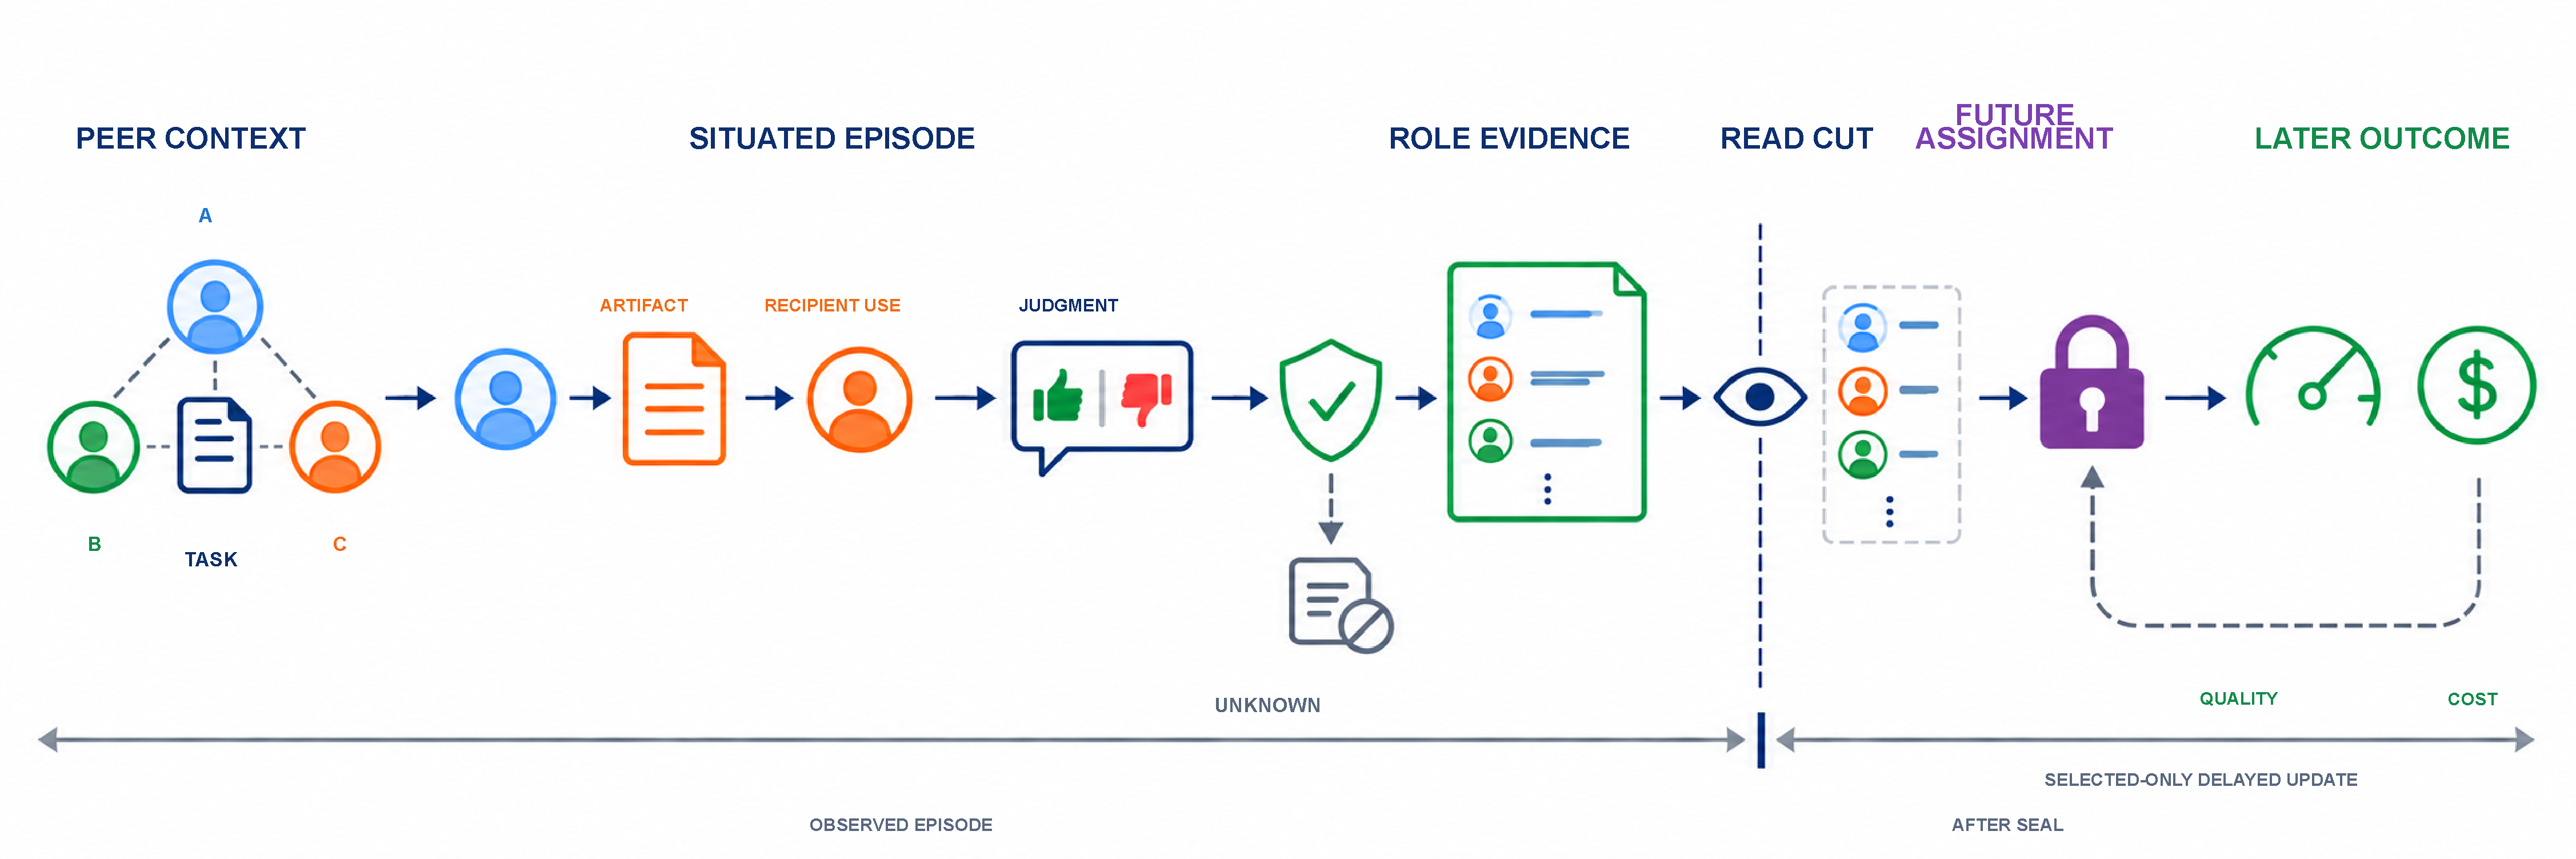
\includegraphics[width=\textwidth]{figures/overview.pdf}
\caption{The earning-roles protocol. Blue marks peer context and the read cut; orange marks situated observation; green marks producer-attributable evidence and the later outcome; violet marks the future assignment. The \textsc{unknown} branch remains audit-only. Gray dashed feedback is delayed and selected-only, entering a future state and next read cut without changing historical evidence or a sealed assignment. Peer-context links are descriptive, not causal.}
\Description{A protocol figure shows peer context, a producer delivery used by a recipient, recipient signal and path evidence, attribution into producer-owned evidence or an audit-only unknown branch, a versioned role ledger, a read cut, exploration followed by a sealed assignment, an independently scored outcome, and delayed selected-only feedback into a future state and next read.}
\label{fig:overview}
\end{figure*}

The following sections define the event and update order, comparison tracks, estimands, and falsification rules.

\section{Related Work and Positioning}

The nearest work differs from our question along three axes: what is observed, when state changes, and whose contribution receives credit. Table~\ref{tab:novelty} makes that boundary explicit. Partner-selection and reputation methods motivate adaptive choice, while graph and role systems motivate changing organization; neither, by itself, identifies whether a concrete producer delivery caused a recipient's action. Recent collaboration benchmarks measure team-level coordination and competition, while interactive agent benchmarks measure environment-level decisions and tool/user outcomes; neither by default turns a recipient's integration trace into a producer-owned label \cite{zhu2025multiagentbench,agashe2025llmcoordination,liu2024agentbench,yao2024taubench}. A contextual-trust or delayed-bandit adapter supplies a strong same-information alternative, not a synonym for the proposed mechanism.

\begin{table*}[t]
\centering\scriptsize
\setlength{\tabcolsep}{3.2pt}
\begin{tabular}{p{0.16\textwidth}p{0.22\textwidth}p{0.19\textwidth}p{0.17\textwidth}p{0.17\textwidth}}
\toprule
Representative method and problem & Observed signal and update & Responsibility / credit semantics & Experimental object & Difference / test here \\
\midrule
Curiosity-Driven Partner Selection; Defection at First Sight \cite{leung2025partner,russell2026partner} & Interaction outcomes; partner state changes after social-game feedback & Peer-level interaction payoff; the cited formulations do not expose a producer--recipient artifact gate & Convention or dilemma games & Versioned delivery use and producer attribution \\
Reputation as a Solution to Cooperation Collapse \cite{ren2026reputation} & Shared assessments and cooperation history; pooled reputation update & Broad reputation/cooperation score; the cited formulation does not expose producer and recipient ownership fields & Language-agent social cooperation & Public responsibility-safe evidence and explicit \unknown{} \\
AgentNet; GPTSwarm \cite{yang2025agentnet,zhuge2024gptswarm} & Agent traces, graph structure, or routing outcomes; organization changes over time & Route/role utility; the cited formulations do not define a producer-artifact credit label & Graph or workflow coordination & Recipient action bound to one delivery and future-owner assignment \\
Dynamic Role Assignment; MoRSE \cite{zhang2026dynamic,li2026morse} & Task context and role/subtask performance; roles or experts are reassigned & Role/expert utility; the cited formulations do not expose producer-artifact attribution inside recipient integration & Debate or mixture-of-experts workflows & Responsibility gate, cross-owner propagation, and delayed correction \\
Finite-time multi-armed bandit \cite{auer2002finite} & Selected-arm rewards; update after an observed arm payoff & Arm-level reward; no producer--recipient ownership contract & Pre-execution selection under observed payoff & Classical selected-reward control; contextual and delayed adapters require separate qualification \\
\bottomrule
\end{tabular}
\caption{Novelty boundary used in the paper. The rows are comparison families, not claims that each source implements the same task. A faithful adapter must preserve the listed visible information, arrival order, selected-only denominator, and complete cost before entering the scientific matrix.}
\label{tab:novelty}
\end{table*}

LLM collaboration frameworks enable workflows, but task success does not resolve artifact ownership \cite{wu2023autogen,zhuge2024gptswarm}. Source judgments precede later assignments; target quality follows execution. Target outcomes may update future decisions but cannot revise a sealed assignment or label the source artifact without independent attribution. Bandit estimators are update comparators, while this protocol tests the timing, ownership, and service cost of that separation.

Cooperative multi-agent learning has long treated credit assignment as a separate problem, using counterfactual advantages or value factorisation to distribute a team payoff \cite{foerster2018coma,rashid2020qmix}. Those methods establish why a shared outcome is insufficient for individual credit, but their reward/state contracts do not identify ownership of a concrete artifact inside a recipient's integration path; this is the boundary tested here.

\section{Problem Formulation}
\label{sec:problem}

\subsection{Objects and information boundary}
At episode $t$, the task supplies context $x_t$ and a legal candidate set $C_t$. The selector chooses one candidate before any candidate in $C_t$ executes:
\begin{equation}
 a_t\sim\pi_{\theta}(\cdot\mid x_t,C_t,R_t),\qquad a_t\in C_t,
 \label{eq:choice}
\end{equation}
where $R_t$ is the public evidence snapshot available at read cut $w_t$. Only the selected candidate is charged for execution. The candidate emits a versioned delivery $o_t$ with digest $d_t$; a recipient $j_t$ reads that delivery and takes action $m_t$. The recipient may accept, revise, reject, or be unable to complete the integration.

The smallest auditable event is
\begin{equation}
 e_t=(x_t,C_t,a_t,o_t,j_t,J_t,m_t,Q_t,Y_t,\tau_t,c_t),
 \label{eq:event}
\end{equation}
where $J_t$ is the recipient judgment, $Q_t$ is the producer-contract check, $Y_t$ is an independent later or terminal outcome when the task defines one, $\tau_t$ is feedback-arrival metadata, and $c_t$ is the complete cost record. The event also stores the candidate version, task/root identifier, artifact digest, feature-schema version, selection probability $p_t=\pi_\theta(a_t\mid x_t,C_t,R_t)$, read-cut digest, and evidence lineage.

\paragraph{Concrete instance.} In the queue case, $x_t$ is the JSON task request, $C_t=\{A,B\}$ is the legal producer menu, and $a_t=B$ selects producer $B$. The delivery $o_t$ is $B$'s versioned priority-module artifact with digest $d_t$; recipient field $j_t=k$ records $k$'s import, test, or repair action as $m_t$; $Q_t$ checks only the producer-owned queue and priority paths; $Y_t$ is the later consumer outcome; and $c_t$ contains model, tool, token, and wall-clock cost.

A repair to $k$'s consumer path remains a publishable, typed handoff observation if complete; it does not create producer-attributable evidence or reward for $B$.

The policy may consume only public events whose arrival is at or before its read cut. Hidden gold, a private scorer, a future target outcome, another policy's state, and an unexecuted candidate cannot affect selection, retry, stopping, or update. A missing event is \unknown{}; a complete but non-attributable event may remain a noisy observation, never a producer-negative label. This boundary is the difference between a role signal and a convenient retrospective score.

\subsection{Observation and attribution gates}
For a source episode, $O_t=1$ requires a frozen contract and registry, sealed pre-action judgment, traceable delivery and recipient action, complete independent checks and terminal outcome, valid identifiers and digests, and completed source lineage. Acceptance, rework, and rejection have equal publication eligibility across their legally paired recipient actions; no arbitrary $J$--action mutation is assumed. Positive or negative checks do not by themselves filter publication. Before completion the judgment is auxiliary only; publication creates a versioned noisy observation and leaves persistent policy state unchanged. Separately, define $G_t=1$ for producer attribution only when all of the following hold: (i) the frozen contract, candidate registry, changed paths, and independent producer check yield a unique producer structural owner (or a pre-registered source defect is uniquely bound to the producer); (ii) the recipient inspected $o_t$ and its action is traceable to $o_t$; (iii) recipient-owned integration paths are empty; (iv) $O_t=1$; and (v) independent defect or quality evidence supports the producer-specific claim. The judge's free-text target role is retained as a calibration observation and its disagreement with the structural owner is logged, but it cannot by itself create or cancel evidence. Otherwise $G_t=0$: its typed observation can remain public, but it cannot create producer evidence or reward.

This gate distinguishes four observations that are often collapsed: a producer-content defect, a recipient's own integration work, a sink or final-task failure, and an unresolved attribution. The public record retains the observation type and the reason for $G_t=0$. A typed observation is not a native evidence identifier: the bridge to a future assignment requires its own qualified binding and is not yet established. This makes safety measurable: a method that refuses ambiguous evidence may have a higher \unknown{} rate while producing fewer false producer penalties.

Figure~\ref{fig:method-state} shows the episode, public-evidence, and local-decision lanes.

\begin{figure*}[t]
\centering
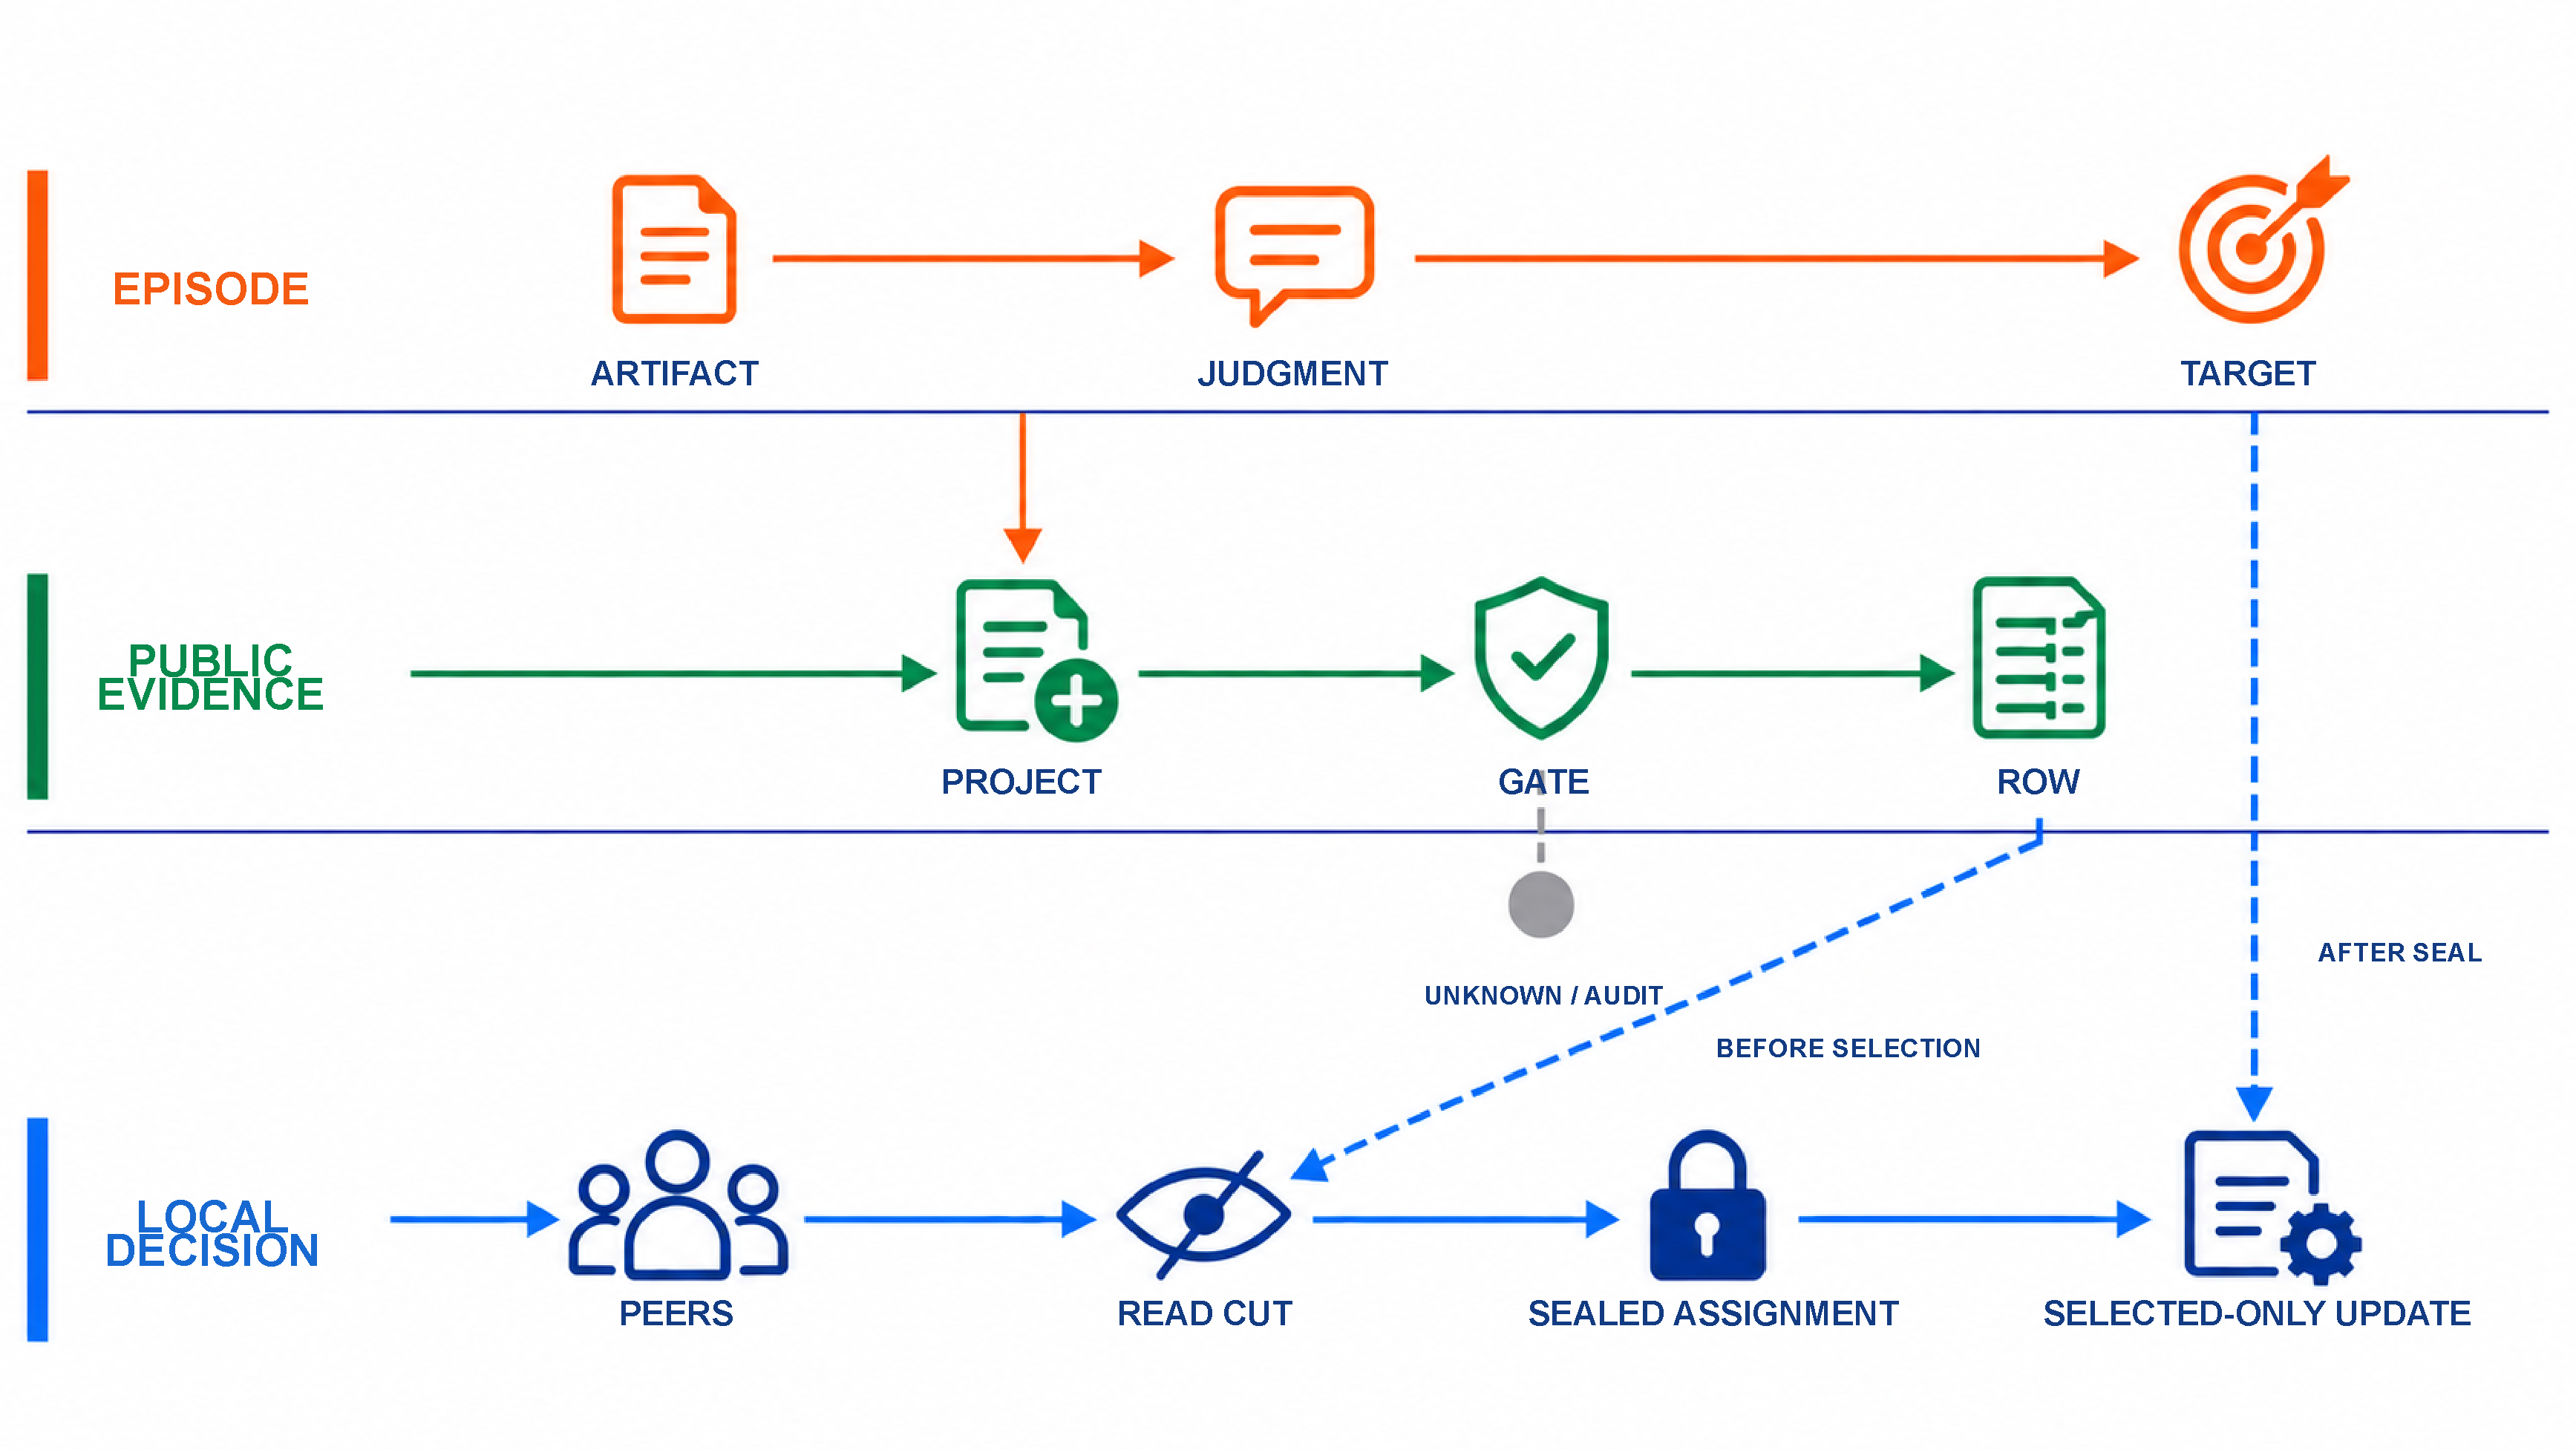
\includegraphics[width=\textwidth]{figures/method_state.pdf}
\caption{Evidence-to-role state. The episode lane records what the producer and recipient actually do; the public-evidence lane projects only typed, responsibility-checked fields; and the local-decision lane reads eligible rows at a read cut before sealing an assignment. Target outcomes arrive after the seal and update only the matching selected opportunity. The representation and updater remain replaceable interfaces.}
\Description{Three horizontal lanes show episode artifacts and judgments, public evidence projection through an ownership and UNKNOWN gate, and a local decision from a candidate menu to a read-cut state, sealed assignment, and selected-only update. Dashed arrows mark evidence eligibility and delayed target outcome.}
\label{fig:method-state}
\end{figure*}

\section{Earning Roles: A Responsibility-Aware Protocol}
\label{sec:method}

The equations below specify the candidate realization used to qualify the protocol interfaces;
they do not lock the final backbone or updater. Those choices remain an experimental question and
will be fixed only after the same-information controls expose the relevant bottleneck.

\subsection{Two-stage evidence and update}
Publication and delayed updating are independent interfaces:
\begin{align}
 \operatorname{publish}(e_t)&\rightarrow \{\text{typed},\;\unknown{},\;\text{invalid}\},\\
 \operatorname{choose}(x_t,C_t,R_t)&\rightarrow (a_t,p_t,\delta_t),\\
 \operatorname{validate}(j_t)&\rightarrow \{\text{credit},\;\unknown{},\;\text{invalid}\},\\
 \operatorname{update}(\text{credit})&\rightarrow \{\text{updated once},\;\text{no-op}\}.
 \label{eq:interfaces}
\end{align}
Publication may change a later assignment's public input, but cannot update persistent policy state. For a later target assignment $j$, ledger binding is necessary but not a reward: credit is legal only if the assignment was written before target selection and task start, the selected candidate and propensity match the sealed preview, the target delivery and outcome are complete, a predeclared responsibility/quality/cost rule passes, and the assignment has not already been credited. The update then evaluates that future responsibility opportunity, never the source episode.

The event-time contract is therefore
\begin{equation}
\begin{aligned}
&\text{source selection}\rightarrow\text{delivery}\rightarrow(Q,J,m,Y)\rightarrow O,G\\
&\rightarrow\text{evidence publication}\rightarrow\text{assignment}\rightarrow\text{target outcome}\\
&\rightarrow\text{delayed selected-only update}.
\end{aligned}
\label{eq:timeline}
\end{equation}
A correction creates a superseding evidence version and affects only future snapshots. Duplicate, late, out-of-order, resource-failed, or invalid events are idempotent no-ops or explicit \unknown{} records. Ledger replay must reproduce the same state digest and choice sequence.

\subsection{Evidence representation and candidate score}
A minimal public state for producer $v$ in context $r$ is
\begin{equation}
 R(v,r)=(n(v,r),s(v,r),u(v,r)),
 \label{eq:state}
\end{equation}
Here $n$ counts typed observations, $s$ summarizes noisy judgment categories without implying producer reward, and $u$ audits unresolved attribution. Count-only or $J$-masked views remove judgment content. A candidate score can combine a task representation $h(x,v,r)$ with the public evidence term:
\begin{equation}
 \operatorname{score}(v\mid x,r)=w^\top h(x,v,r)+\beta\frac{s(v,r)}{n(v,r)+\alpha}.
 \label{eq:score}
\end{equation}
For the queue instance, $r$ is the priority-contract context, $h(x,B,r)$ is the fixed task--candidate representation for producer $B$, and $n,s,u$ summarize versioned observations and their attribution flags. A recipient-only repair can remain in $n$ and $u$ as a typed observation; it cannot supply producer reward for $B$.

The representation $h$, updater, and constants are replaceable implementation conditions rather than the scientific object. The score is a contract-level construction, not a theorem or a claim that one backbone is optimal. The selector uses a pre-registered exploration floor, records $p_t$, and uses preview--assignment--commit so that writing a future assignment cannot resample the selected candidate.

The same protocol yields three observable predictions. First, responsibility safety is measured by false producer-attribution and \unknown{} rates under recipient-only interventions. Second, temporal validity is measured by read-cut and assignment-order invariants and by the absence of target-outcome fields at selection. Third, bounded online service is measured by per-event update latency, backlog, state bytes, and complete cost. These predictions map to the RQ2--RQ4 endpoints; they are not assumptions that the score automatically satisfies.

\subsection{Executable selector and update contract}
A candidate selector uses a frozen encoder for tasks, public profiles, and published observations. To avoid reusing a training label, it separates a timestamped profile from later evidence:
\begin{align}
 P_{v,k}&=\operatorname{summarize}\{e_i:O_i=1,\;t_i<\kappa_k\},\\
 D_{v,k,t}&=\operatorname{summarize}\{e_i:O_i=1,\;\kappa_k\leq t_i\leq w_t\},\\
 z_t(v)&=[\phi(x_t)\,\|\,\phi(P_{v,k})\,\|\,\phi(D_{v,k,t})\,\|\,b(v)] .
 \label{eq:selector-state}
\end{align}
Here $\kappa_k$ is the profile cut, $w_t$ the legal read cut, $\phi$ frozen, and $b(v)$ public version and uncertainty features. Empty inputs remain explicit; each event enters at most one of $P$, $D$, or target credit.

The candidate distribution is
\begin{equation}
 q_t(v)=\operatorname{softmax}_{v\in C_t}\left(g_\psi(z_t(v))+\theta_v^\top\phi(x_t)\right),
 \qquad a_t\sim q_t,
 \label{eq:selector}
\end{equation}
Here $g_\psi$ is a candidate fixed head and $\theta_v$ a residual updated only after a selected assignment passes the independent reward contract. Head, exploration, clipping, and learning rate are fixed before confirmation; profile-only, delta-only, residual-only, and no-history controls isolate components.

The candidate runtime contract requires five auditable operations. (1) It appends the sealed source judgment, publishes a complete typed observation, and checks attribution separately; incomplete records become \unknown{}. (2) It advances a read watermark and materializes a state snapshot, recording the feature-schema and state digest. (3) It scores only the legal candidate menu and writes the candidate set, probabilities, sampled action, and assignment digest before the target starts. (4) When the target outcome arrives, it verifies the matching assignment, selected-only eligibility, version, idempotency key, and independent reward contract. (5) It applies one bounded residual update and emits a new state digest; profile and delta materialization wait for the next declared read cut. The sequence is required to permit replay after a crash without changing a sealed choice.

\begin{table}[t]
\centering\scriptsize
\setlength{\tabcolsep}{2pt}
\caption{State fields and their legal update event. A field is read only after its listed cut and never retroactively edits a sealed assignment.}
\label{tab:state-contract}
\begin{tabular}{p{.25\columnwidth}p{.25\columnwidth}p{.38\columnwidth}}
\toprule
Field & Source & Update boundary \\
\midrule
Profile $P_{v,k}$ & Published typed observations before $\kappa_k$ & Next profile cut; immutable thereafter \\
Delta $D_{v,k,t}$ & New typed observations after $\kappa_k$ & Read watermark $w_t$ \\
Residual $\theta_v$ & Validated selected target reward & Matching delayed update only \\
Uncertainty $u(v)$ & Unknown, duplicate, or correction records & Monotone audit update \\
Assignment $a_t,p_t$ & Candidate menu and snapshot & Sealed before target execution \\
\bottomrule
\end{tabular}
\end{table}

This candidate contract makes late judgments visible only to future snapshots, excludes recipient repair from producer reward, and leaves missing outcomes without updates. Confirmation must measure latency, state size, and utility; if a calibrated control matches it at equal information and cost, no fusion gain is claimed.

\section{Benchmark and Baselines}
\label{sec:benchmark}

\subsection{Two complementary tracks}
The primary track, \textbf{ArtifactRole}, is a TeamBench-derived candidate benchmark \cite{kim2026teambench}. It contains producer artifacts, recipient dependencies, use/rework/rejection actions, responsibility checks, later assignments, downstream adoption, and complete cost. Candidate roots are DIST1 queue-race (development diagnostic) and PIPE3 stream-processing (conditional confirmation); renamed seeds are not independent roots. Promotion requires material visibility, write permissions, scorer coverage, root independence, and clean replay. This stricter contract is intentional: TeamBench's role separation supplies the dependency scaffold, while ArtifactRole adds the producer--recipient attribution and future-assignment fields needed by our question.

Producer conformance and terminal usability are scored separately: a recipient may normalize a nonconforming delivery into a usable result. Every executed arm, including no-update, receives terminal evaluation. A prior valid, evidence-bound assignment and an independently validated reward are required for assignment credit, not for inclusion in the outcome denominator; native benchmark conformance remains a separate endpoint.

The secondary \textbf{PeerSelect} track uses a pinned local graph interaction benchmark for selected-only payoff, local candidate sets, online updates, drift, and service cost. It isolates update behavior but cannot establish situated artifact judgment or producer attribution. The tracks share event and selector interfaces while keeping tasks, labels, scorers, denominators, and claims separate.

\subsection{Predeclared baselines}
All primary arms receive the same candidate menu, initial opportunities, model/API/tool budget, exploration opportunity, feedback arrival schedule, failure handling, and complete cost accounting. Each arm reads only its legal history. Table~\ref{tab:baselines} names the alternative explanations that the matrix must rule out.
\begin{table*}[t]
\centering\small
\begin{tabular}{p{0.18\textwidth}p{0.38\textwidth}p{0.32\textwidth}}
\toprule
Arm & Read/update contract & Alternative explanation tested\\
\midrule
Uniform & Candidate menu; fixed local-uniform sampling & Random allocation and exploration lower bound\\
No update & Initial prior and current context; feedback ignored & Static execution is sufficient\\
Raw acceptance & Recipient accept/reject only & Responsibility filtering adds no value\\
Terminal only & Independent final outcome only & Situated judgment adds no information\\
Contextual trust/bandit & Same context, judgment, propensity, delay, and budget as RARE & The effect is ordinary contextual trust or bandit learning\\
Pooled controller & Permitted public history under the same total capacity & A shared controller explains the gain\\
Closest published adapter & Faithful public-information adapter, if it passes qualification; otherwise an explicit \textsc{no-go} cell & Existing role/organization method is sufficient\\
RARE & Typed observations, attribution checks, and validated delayed credit & Candidate closed-loop mechanism\\
\bottomrule
\end{tabular}
\caption{Primary comparison boundary. A named arm enters the scientific matrix only after an executable adapter, information declaration, cost contract, and independent qualification pass.}
\label{tab:baselines}
\end{table*}

If the closest published method cannot preserve the same public fields, candidate menu,
arrival order, selected-only rule, and complete-cost contract, the confirmation card records
an explicit \textsc{no-go}; it does not replace that missing adapter with a self-authored
weak control.

RLS, online logistic/SGD, periodic refitting, and any candidate incremental updater are training comparators. They are not counted as separate selection policies and are not presented as the innovation merely because they are fast. The contextual-trust arm follows the same information contract as classical contextual bandits \cite{li2010contextual}; its delay handling is compared with the general delayed-feedback setting \cite{joulani2013delayed}. Agent ranking and human--LLM teaming provide additional positioning points, but neither substitutes for the producer--recipient label contract \cite{lanctot2025soft,yurrita2026guidelines}.

\section{Experimental Questions and Matrix}
\label{sec:experiments}

The matrix below is a pre-specified design scaffold, not an observed result table. A cell enters
the confirmation analysis only after its root, stream, seed, budget, scorer, cost contract,
stopping rule, and manifest digest are frozen before the corresponding calls; otherwise it
remains planned or \unknown{}.

\subsection{Research questions and estimands}
\textbf{RQ1 (information value).} Does an eligible situated judgment predict an independent producer-contract or later-use result beyond raw acceptance and terminal-only feedback? The primary estimands are out-of-sample log loss, Brier score, AUC when defined, calibration, and incremental predictive value on an independent root. The confirmation card also freezes a field-level feature manifest: a judgment-only view, a producer-check/terminal-only view, and their declared fusion. Artifact, structural owner, Qp, Y, read cut, arrival schedule, and cost remain fixed while legally paired recipient-judgment/action variants test whether the assignment or score actually responds to J.

\textbf{RQ2 (assignment causality).} Does public evidence change an assignment made before target execution, including when the future owner did not produce the source judgment? We measure assignment-change probability, propensity-weighted future quality, adoption, rework, and complete cost. Evidence from producer $B$ cannot be consumed as if it belonged to producer $C$.

\textbf{RQ3 (online behavior).} Does the update path satisfy the service contract under selected-only delayed feedback? We report publish, read/assignment, and update p50/p95 latency, service lag, backlog, state bytes, CPU/GPU/RAM, token/tool/API calls, and replay time.

\textbf{RQ4 (stability and boundaries).} How does the method behave under task or peer drift, delayed or out-of-order feedback, version replacement, recipient-only work, mixed ownership, scorer failure, and resource failure? We report old-root peak and mean forgetting, drift recovery window, \unknown{} rate, correction consistency, and false producer attribution.

The primary unit of uncertainty is an independently reset stream. Episodes inside one stream are dependent. We use paired stream-level estimates, bootstrap or randomization intervals over streams, and pre-registered multiplicity control for the primary contrasts. Missing, invalid, or unknown events remain in the denominator and are never silently recoded as failures or successes.

\paragraph{Primary endpoint design.} The design reserves four card identifiers: \texttt{H1} uses independent-target Brier score (lower is better) for incremental situated signal; \texttt{H2} uses future assignment quality--complete-cost utility (higher is better) against the same-information control; \texttt{H3} uses selected-feedback update p95 latency and backlog under the fixed arrival budget (lower is better); and \texttt{H4} uses false producer-attribution rate under ownership mutations (lower is better). Each card is required to fix its control, minimum practically important difference or precision target, exploration floor/positivity condition, stream-level 95\% interval, and stopping rule before outcomes are observed; the current design-only manifest records which fields remain unfrozen.

Only these H1--H4 endpoints are primary for the headline interpretation. The remaining measures in the matrix are secondary or exploratory and cannot be promoted after outcomes are observed.

\subsection{Complete experiment matrix}
Table~\ref{tab:matrix} is the execution skeleton. The result columns are deliberately empty; the confirmation manifest must bind every row to a root, split, policy, seed, budget, scorer, and raw log before any result is filled.
\begin{table*}[t]
\centering\scriptsize
\begin{tabular}{p{0.08\textwidth}p{0.12\textwidth}p{0.14\textwidth}p{0.18\textwidth}p{0.20\textwidth}p{0.12\textwidth}}
\toprule
RQ/cell & Track/root & Policy/intervention & Primary comparison & Measures & Result\\
\midrule
RQ1-I & ArtifactRole / dev root & raw acceptance vs terminal only vs RARE & Same producer deliveries and recipient observations; legal feedback only & Brier/log loss, calibration, judge reliability & \blank\\
RQ1-II & ArtifactRole / confirmation root & contextual trust vs RARE & Same public read cut, delay, propensity, model and budget & Incremental prediction and cross-root transfer & \blank\\
RQ2-I & ArtifactRole / confirmation root & no evidence vs public evidence only & Preview--assignment before target execution & Assignment change, future quality, adoption, rework & \blank\\
RQ2-II & ArtifactRole / confirmation root & delayed update only vs public evidence + delayed update & Same target tasks and selected-only outcome & Future utility and complete cost & \blank\\
RQ2-III & ArtifactRole / confirmation root & RARE vs pooled controller & Same total public capacity and candidate menus & Quality--cost utility, concentration, propensity & \blank\\
RQ3-I & PeerSelect / dev streams & uniform, no-history, history-only, candidate updater & Local graph, selected-only payoff, fixed call/token budget & Regret/payoff, update p50/p95, state bytes & \blank\\
RQ3-II & PeerSelect / drift streams & updater with/without correction and replay & Pre-registered peer/task drift and delayed feedback & Recovery window, forgetting, backlog, replay equality & \blank\\
RQ4-I & ArtifactRole / all qualified roots & responsibility mutation matrix & Producer-only, recipient-only, mixed, unknown, resource failure & False attribution, UNKNOWN precision, no-op rate & \blank\\
RQ4-II & ArtifactRole / all qualified roots & leave-one-mechanism-out & Remove gate, public evidence, delay, locality, or updater & Main utility, safety, cost, interaction effect & \blank\\
\bottomrule
\end{tabular}
\caption{Pre-specified experiment matrix. Each row binds a research question to a root, split, policy, seed, budget, scorer, cost record, and raw event manifest before interpretation; a row is not an observed result until its confirmation card is frozen and executed.}
\label{tab:matrix}
\end{table*}

Figure~\ref{fig:experiment-map} links the two tracks to the four research-question endpoints; it does not merge their labels or claims.

\begin{figure*}[t]
\centering
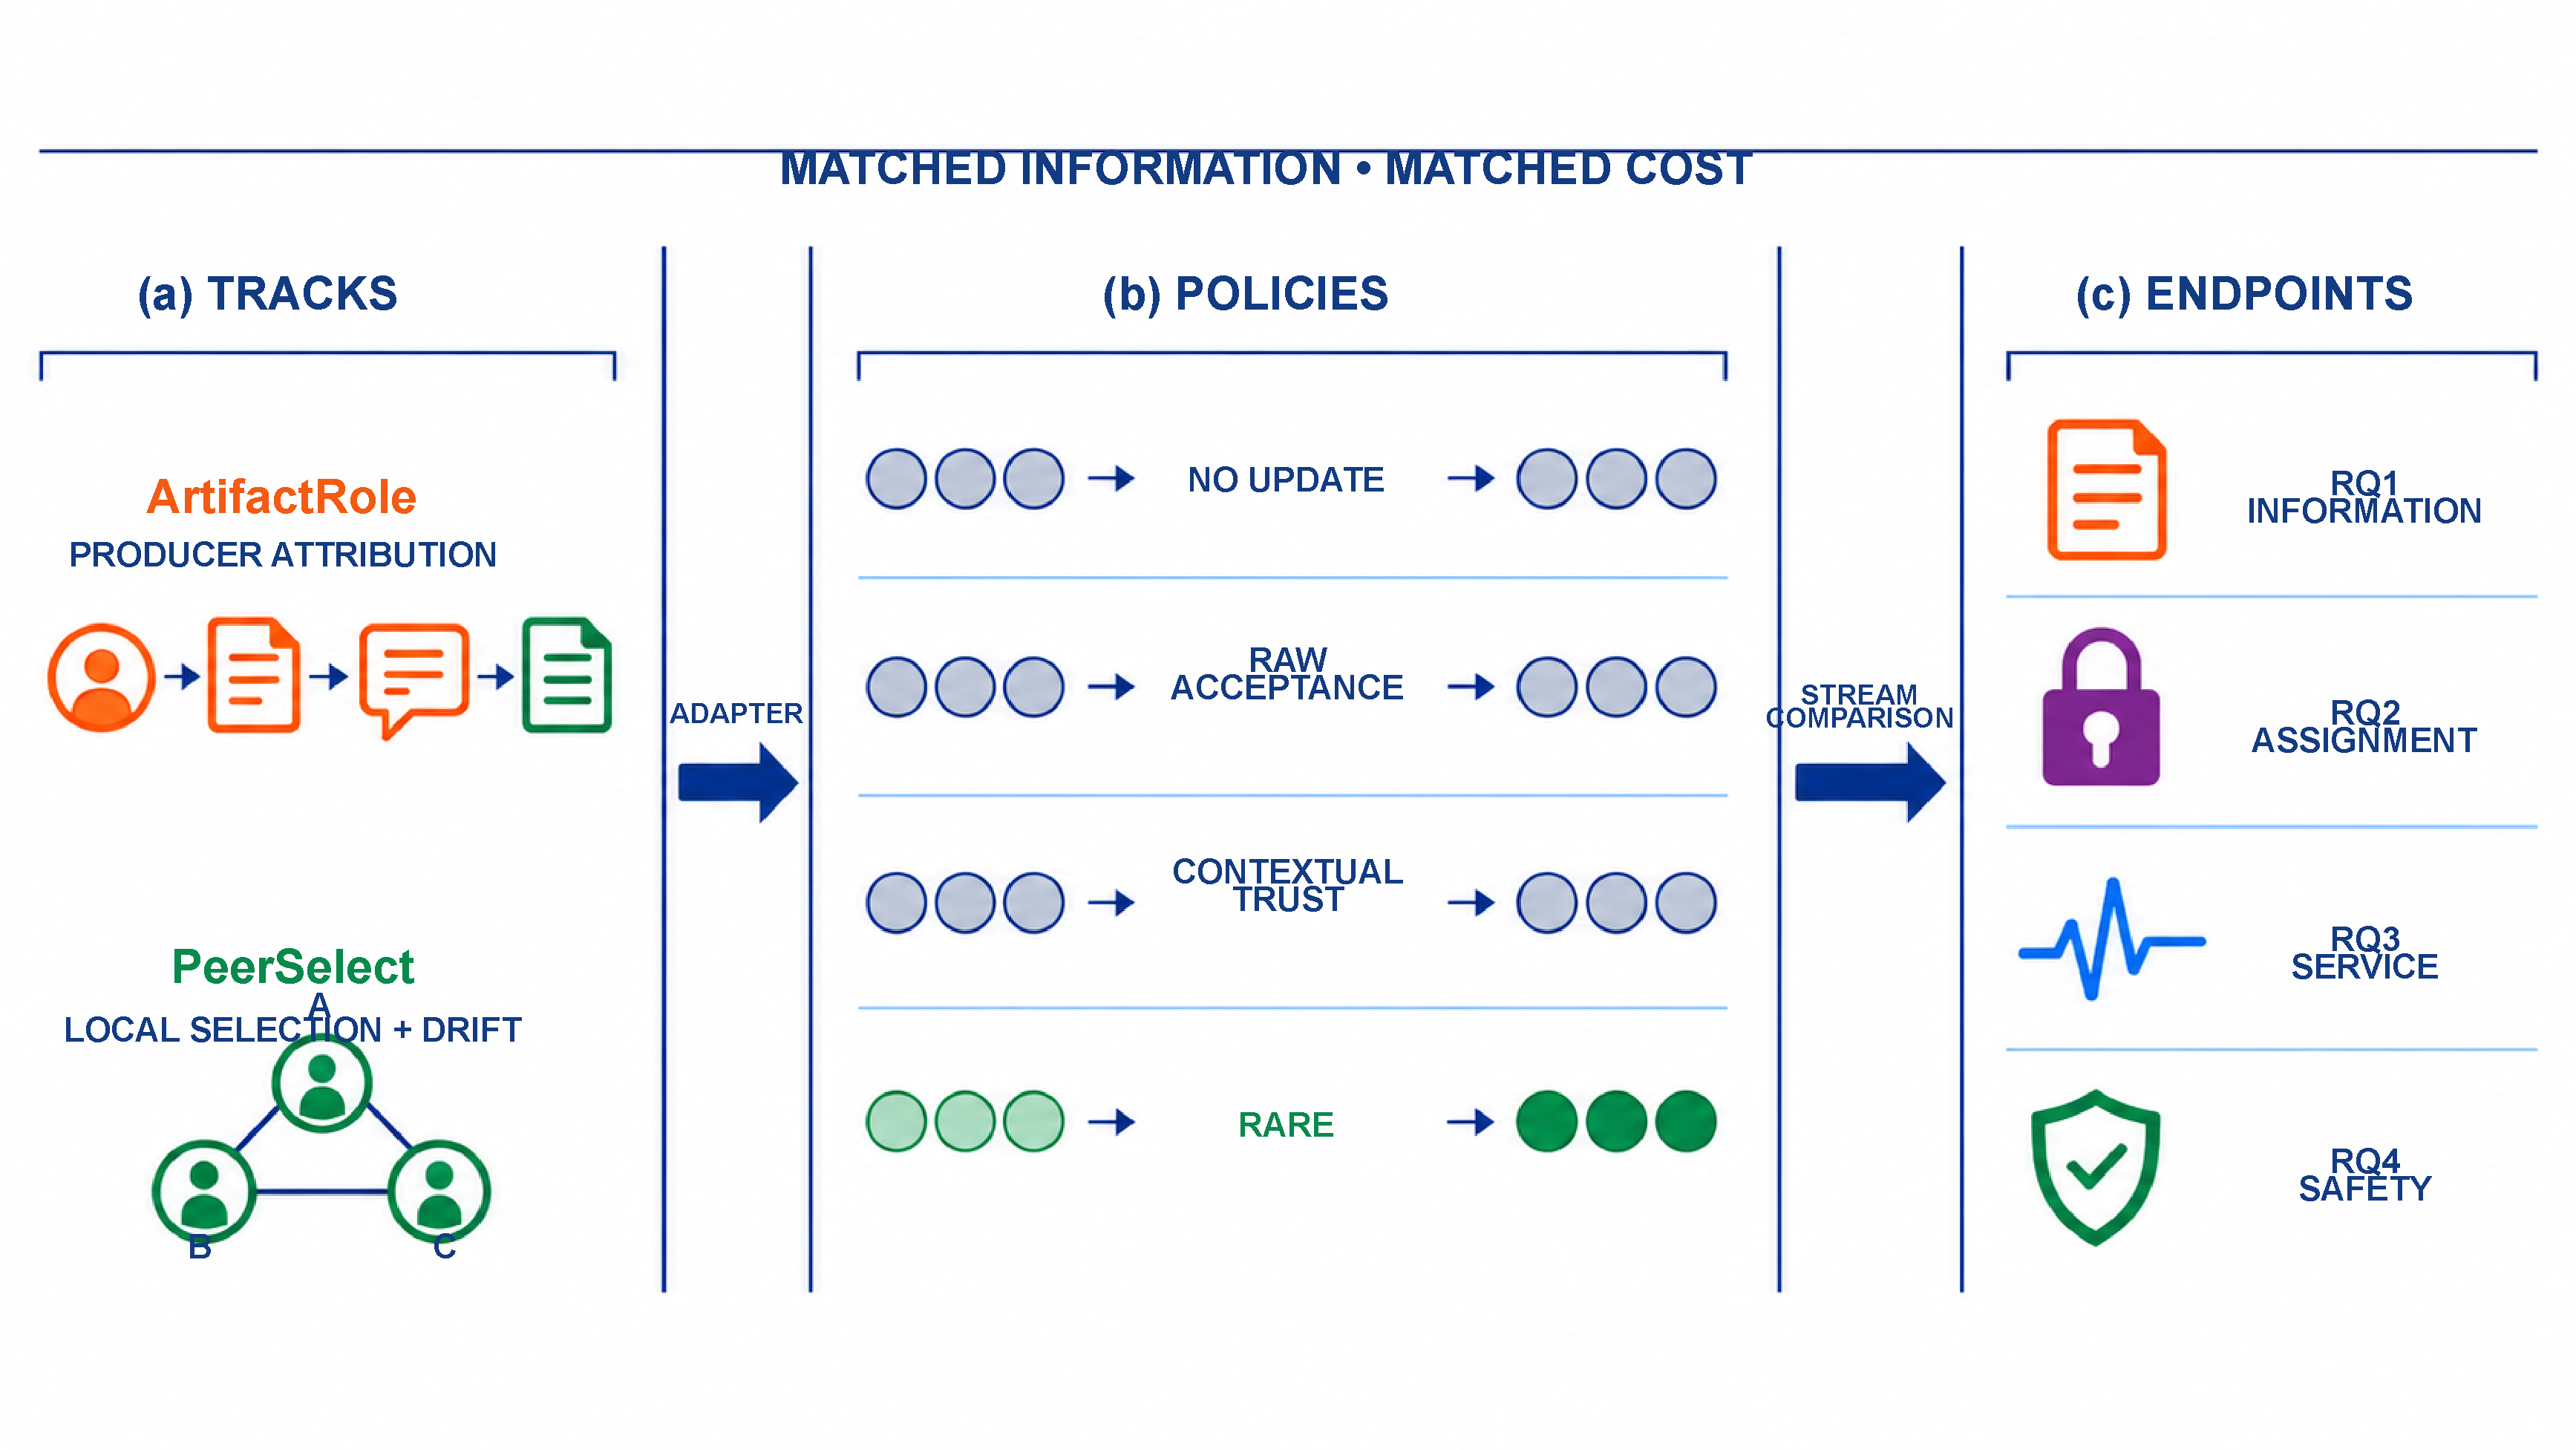
\includegraphics[width=\textwidth]{figures/experiment_map.pdf}
\caption{Experiment map. ArtifactRole measures the situated producer--recipient phenomenon; PeerSelect isolates local selection, drift, and service cost. All policy arms receive the same candidate menus, lawful feedback schedule, task opportunities, and complete-cost budget before the four research questions are scored.}
\Description{A three-panel map from the ArtifactRole and PeerSelect tracks to matched policy arms and four research-question endpoints: information, assignment, latency and cost, and safety and drift.}
\label{fig:experiment-map}
\end{figure*}

Table~\ref{tab:headline} reserves the endpoints that will carry the paper's headline comparison once the confirmation manifest is complete.
\begin{table}[t]
\centering\small
\caption{Headline endpoints. Values are supplied only by the frozen confirmation manifest; intervals are stream-level 95\% intervals.}
\label{tab:headline}
\begin{tabular}{p{.28\columnwidth}p{.17\columnwidth}p{.17\columnwidth}p{.17\columnwidth}}
\toprule
Endpoint & RARE & Best same-information arm & Difference / interval\\
\midrule
Future quality & \blank & \blank & \blank\\
Complete cost & \blank & \blank & \blank\\
Quality--cost utility & \blank & \blank & \blank\\
Assignment change & \blank & \blank & \blank\\
Judgment Brier score & \blank & \blank & \blank\\
Update p95 / state bytes & \blank & \blank & \blank\\
Old-root forgetting & \blank & \blank & \blank\\
UNKNOWN / false attribution & \blank & \blank & \blank\\
\bottomrule
\end{tabular}
\end{table}

\subsection{Budget, statistics, and reporting}
Every model request reserves attempted calls, prompt tokens, maximum completion tokens, tool time, and storage before dispatch; errors release only unused reservations and retain their observed cost. We charge producer execution, recipient integration, judgment service, communication, retries, replay, verification, and returned artifacts. Development/search cost is reported separately from deployment cost. A pooled controller receives the same total capacity, and arms that do not use a judgment still pay the declared comparison cost or use a shared judgment call whose output is masked.

For each stream we record configuration, model route and version metadata, code and data hashes, seed, hardware, timestamps, raw API responses, token usage, intermediate actions, failure traces, \unknown{} reasons, and per-sample outcomes. We report means and medians with 95\% stream-level intervals, effect sizes for pre-registered contrasts, per-root heterogeneity, ITT and per-protocol denominators, and quality--cost Pareto points. The main endpoint is assignment-level future quality--complete-cost utility; source producer score is auxiliary and cannot replace it.

For every primary contrast, the experiment card fixes the direction, minimum practically important difference or precision target, stream-level 95\% interval, and stopping rule before confirmation. A row without those fields is a design specification rather than an interpretable result.

\subsection{Ablations and falsification}
A count-only/$J$-masked control holds the same published handoffs and costs while removing judgment-category information. The minimum ablation grid is: (A) no evidence/no update; (B) public evidence only, with persistent state unchanged; (C) delayed update only, without new public evidence; and (D) public evidence plus delayed update. Additional interventions remove responsibility filtering, selected-only restriction, delay, locality, correction/replay, or the assignment binding one at a time while holding information, model, candidate menu, and budget fixed. A content mutation that changes a visible judgment while holding terminal quality fixed must change the comparator score if the comparator actually consumes that judgment.

The main claim is withdrawn if an observation publication implicitly changes persistent policy; if a recipient repair is credited to a producer; if assignment or read-cut order is invalid; if unknown or duplicate events update state; if contextual trust explains the complete effect; or if gains disappear at matched complete cost. A null, a trade-off, or a qualified protocol result is scientifically valid, but it cannot be written as successful role formation.

\subsection{Reproducibility and reporting}
Before execution, each experiment card fixes the matrix cell, root, stream, model, budget, scorer, estimand, and stopping rule. A hash-linked ledger connects every aggregate to its raw calls and per-episode outcomes. Failed attempts retain their observed cost; incomplete cells remain \textsc{tbd}, never zero. We report safety without utility gain as a safety result, and prediction without changed future assignment as an information result. Neither alone establishes role formation.

\section{Results and Evidence Boundary}
\label{sec:current}

\textbf{RQ1--RQ2 (information and assignment).} The confirmation card will fill the held-out Brier score, matched-information comparison, assignment-change rate, and future quality--cost utility in Tables~\ref{tab:headline} and~\ref{tab:matrix}: \textsc{tbd}. Prediction without a sealed future assignment supports an information claim only; assignment without an independent target outcome does not establish responsibility transfer.

\textbf{RQ3--RQ4 (service and safety).} The latency, backlog, state-size, forgetting, \unknown{}, and false-attribution cells remain \textsc{tbd}. We will interpret a safe null, a quality--cost trade-off, and a qualified positive result as different claims rather than as interchangeable evidence.

Current development traces expose attribution and measurement hazards, but do not establish predictive utility, future assignment gains, or real-time learning. No confirmation cell is filled from these traces. Results require qualified roots, independent streams, matched baselines, and complete cost.

\section{Discussion and Limitations}

The mechanism addresses responsibility opportunities in tasks with an actual producer--recipient dependency. It does not establish general expertise or autonomous workflow discovery. PeerSelect can isolate local adaptation, but cannot replace ArtifactRole's attribution evidence; conversely, an ArtifactRole result cannot be interpreted as general bandit performance.

Judge error, selective exposure, root dependence, incomplete responsibility coverage, and judgment cost threaten validity. We therefore preserve \unknown{} events, log selection propensities, assess judge reliability, and evaluate independent roots and streams. Terminal usability also differs from producer conformance: successful downstream normalization need not vindicate an upstream contract violation. Neither metric alone identifies the producer's contribution to future team utility.

Backbone and updater selection remains an empirical question. Frozen representations with incremental heads, online logistic/RLS updates, and periodic refitting are matched candidates. Latency alone cannot establish useful adaptation: a fast update may reinforce a misattributed label or forget previously useful distinctions. The drift and old-task evaluations must accompany update timing before a real-time learning claim is supported.

Deployment must expose refusals to learn, preserve correction lineage, and retain enough provenance to replay decisions after evidence compression. Tool selection can share this event interface, but requires its own execution oracle; peer judgments retain the ownership gate. The release will include versioned code, prompts, scorer contracts, raw-event manifests, and table-generation scripts. Offline replay reconstructs decision order; reproducing API latency and token costs requires fresh calls. These boundaries distinguish an executable protocol from demonstrated improvements in role formation.

\section{Conclusion}

This paper defines a precise object for self-evolving multi-agent roles: a recipient's situated judgment becomes a typed noisy observation, producer attribution is checked separately, and a later sealed assignment is evaluated with independent quality and complete cost. The protocol makes each arrow auditable and gives close alternatives the same information and budget. The current draft records the method contract, benchmark and baseline matrix, statistical plan, and falsification boundary while leaving empirical cells empty. The decisive result will be whether the complete loop improves future responsibility allocation beyond equally informed alternatives without sacrificing attribution safety, online service, stability, or cost.

\clearpage
\bibliographystyle{ACM-Reference-Format}
\bibliography{references}
\end{document}
